% Chapter 1

\chapter{Introducción General} % Main chapter title

\label{Chapter1} % For referencing the chapter elsewhere, use \ref{Chapter1} 
\label{IntroGeneral}

%----------------------------------------------------------------------------------------

% Define some commands to keep the formatting separated from the content 
\newcommand{\keyword}[1]{\textbf{#1}}
\newcommand{\tabhead}[1]{\textbf{#1}}
\newcommand{\code}[1]{\texttt{#1}}
\newcommand{\file}[1]{\texttt{\bfseries#1}}
\newcommand{\option}[1]{\texttt{\itshape#1}}
\newcommand{\grados}{$^{\circ}$}

%----------------------------------------------------------------------------------------

%\section{Introducción}

%----------------------------------------------------------------------------------------
\section{Descripción general del trabajo y conceptos claves}

El trabajo desarrollado consiste en un sistema adquisidor de datos con los sensores necesarios para una medición de potencia eléctrica, en otras palabras un medidor digital de energía eléctrica.

La adquisición de datos o adquisición de señales consiste en la toma de muestras del mundo real (sistema analógico) para generar datos que puedan ser manipulados por un ordenador u otros dispositivos electrónicos (sistema digital). Consiste en tomar un conjunto de señales físicas, convertirlas en tensiones eléctricas y digitalizarlas de manera que se puedan ser procesadas por una computadora. Se requiere una etapa de acondicionamiento, que adecua la señal a niveles compatibles con el elemento que hace la transformación a señal digital.\citep{NIDataAdquisition}

Las mediciones eléctricas son los métodos, dispositivos y cálculos usados para medir cantidades eléctricas. La medición de cantidades eléctricas puede hacerse al medir parámetros eléctricos de un sistema. Usando transductores, propiedades físicas como la temperatura, presión, flujo, fuerza, y muchas otras pueden convertirse en señales eléctricas, que pueden ser convenientemente registradas y medidas. \citep{MEcitation}

Un convertidor de señal analógica a digital es un dispositivo electrónico capaz de convertir una señal analógica, ya sea de tensión o corriente, en una señal digital mediante un cuantificador y codificándose en muchos casos en un código binario en particular. Donde un código es la representación unívoca de los elementos, en este caso, cada valor numérico binario hace corresponder a un solo valor de tensión o corriente.\citep{ADCcitation}


\subsection{Sistemas electrónicos para mediciones eléctricas}

Las aplicaciones mas tempranas de computadores digitales a problemas de sistemas de potencia datan alrededor de 1940. La mayoría de las aplicaciones tempranas estaban limitadas en alcance debido a la pequeña capacidad de las tarjetas de las calculadoras usadas en ese periodo. Computadoras digitales de larga escalas estuvieron disponibles a mediados de 1950, y el éxito inicial de programas de flujo de carga llevaron al desarrollo de programas para cálculos de corto circuitos y estabilidad.\citep{761852}

Hoy en día la computadora digital es una herramienta indispensable en el planeamiento de sistemas de potencia, en el que es necesario predecir el crecimiento futuro y simular operaciones día  a día sobre períodos de 20 años o más.\citep{761852}

Los medidores electrónicos miden energía usando varios componentes altamente integrados o un circuito integrado especifico. Estos dispositivos digitalizan el voltaje instantáneo y la corriente vía un ADC sigma delta  de alta resolución. La técnica de diseño de estos medidores digitales es influenciada por tres grandes factores tales son el costo deseado, eficiencia y tamaño total. Mientras que el costo esta influenciado por la capacidad de compra del cliente, la eficiencia y el tamaño deben cumplir estrictamente con los estándares.\citep{articleDM}

Las mediciones digitales de potencia y energía eléctrica están basadas en el muestreo y digitalización de valores instantáneos de voltaje y corriente en intervalos regulares de tiempo. Tal medición de potencia y energía se encuentra influenciada no solo por las inexactitudes del circuito analógico pero sino también de las inexactitudes del proceso de muestreo en si mismo.

La exactitud del medidor eléctrico digital depende en la exactitud del circuito analógico de entrada analógica, la exactitud del conversor analógico-digital y la exactitud de los cálculos digitales.\citep{Hribik2004DigitalPA}

\section{Motivación}

En la actualidad se pueden encontrar en el mercado internacional múltiples módulos electrónicos con puertos de comunicación para la medición de energía eléctrica como así también medidores digitales de energía de diferentes marcas para diferentes entornos, los que nos permite pensar que un dispositivo similar podría ser fabricado en la Argentina.

\begin{figure}[h]
	\centering
	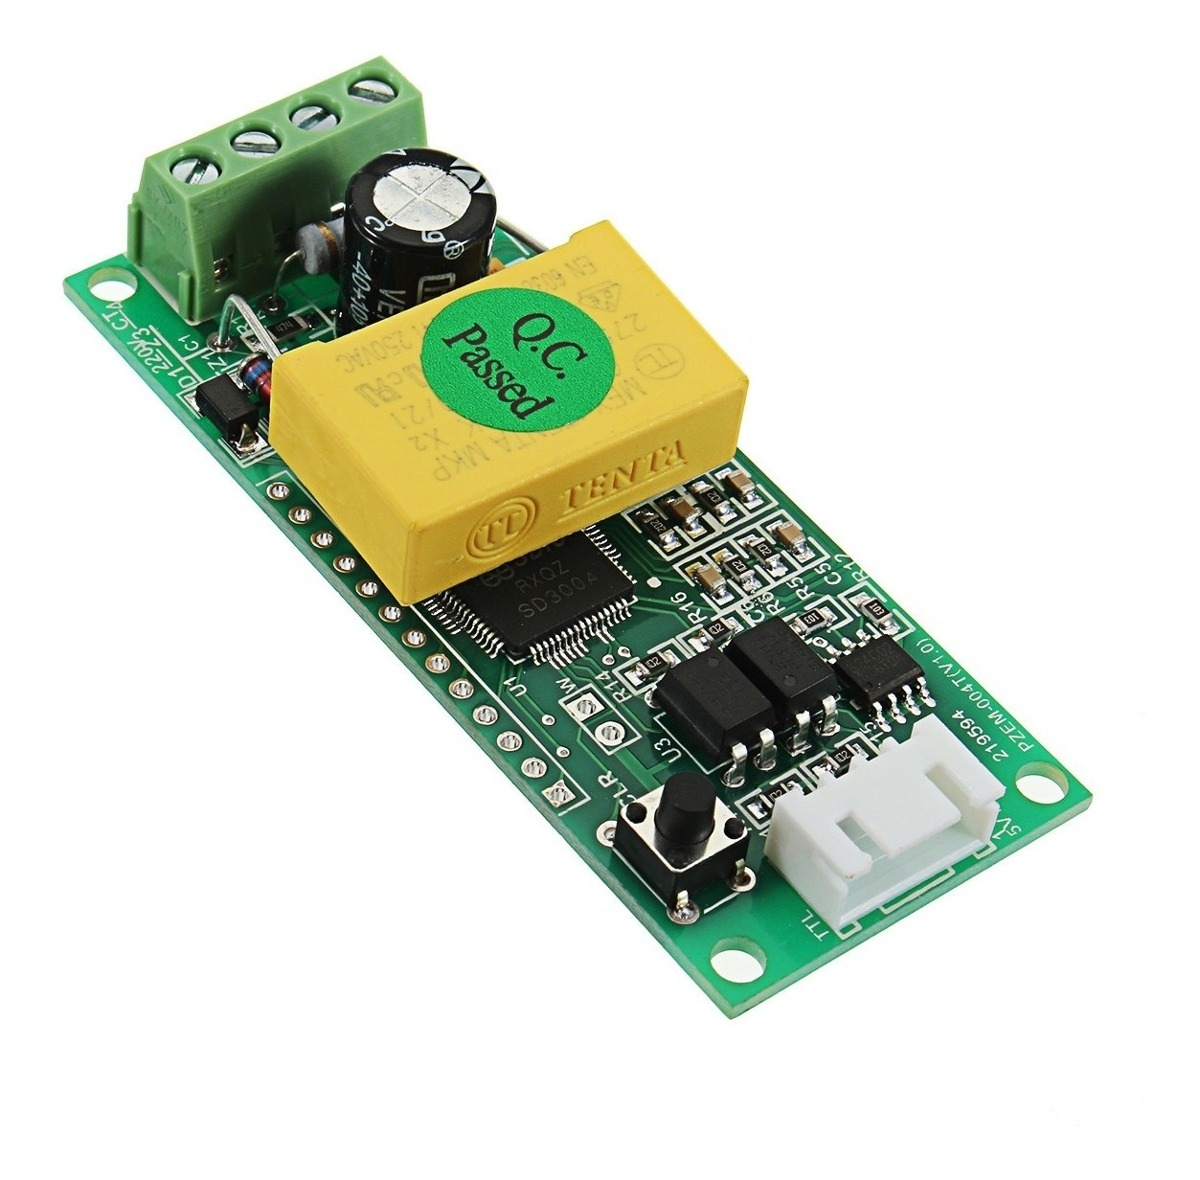
\includegraphics[width=80mm,keepaspectratio]{Figures/pzeem004.jpg}
	\caption{Modulo de medicion de energia electrica con comunicacion serie universal.}
	\label{fig:texmaker}
\end{figure}

%----------------------------------------------------------------------------------------






